[114 r\textsuperscript{o}] arctius est. Ideo et pondus\protect\index{Sachverzeichnis}{pondus} liquoris\protect\index{Sachverzeichnis}{liquor} in \textit{ab} tanto fortius \edtext{resistet}{\lemma{fortius}\Afootnote{ \textit{ (1) }\ erit \textit{ (2) }\ resistet \textit{ L}}}. \edtext{Ergo in exercitio vis Elasticae}{\lemma{resistet.}\Afootnote{ \textit{ (1) }\ Ergo si in fir \textit{ (2) }\ Ergo  \textit{(a)}\ liquores\protect\index{Sachverzeichnis}{liquor|textit} vim Elasticam\protect\index{Sachverzeichnis}{vis!elastica|textit} \textit{(b)}\ in exercitio vis Elasticae \textit{ L}}} quoque liquorum\protect\index{Sachverzeichnis}{liquor} non minus quam \hspace{1pt}gravitatis\protect\index{Sachverzeichnis}{gravitas},\hspace{1pt} nihil\hspace{1pt} ad\hspace{1pt} rem\hspace{1pt} pertinebit\hspace{1pt} crassities.\hspace{1pt} Jam\hspace{1pt} in  
%Zeitz auskommentiert \startlock
%\begin{center}                                    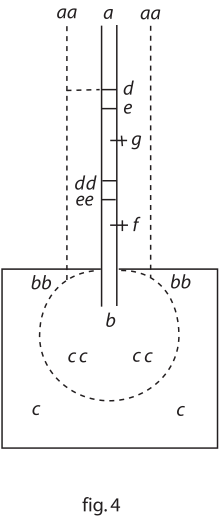
\includegraphics[width=0.28\textwidth]{images/37_4_114r}\\\textit{[Fig. 5]}
%                        %\caption{Bildbeschreibung}
%                        \end{center}\endlock
%                        %@ @ @ Dies ist eine Abstandszeile - fuer den Fall, dass mehrere figures hintereinander kommen, ohne dass dazwischen laengerer Text steht. Dies kann zu einer Fahlermeldung fuehren. @ @ @ \\
%                        exercitio vis Elasticae\protect\index{Sachverzeichnis}{vis!elastica} 
                        \edtext{sive liquidorum sive solidorum}{\lemma{}\Afootnote{sive liquidorum sive solidorum \textit{ erg.} \textit{ L}}} in universum\protect\index{Sachverzeichnis}{universum}, \edtext{suspensio ponderis altitudine ejus non variatur}{\lemma{universum,}\Afootnote{ \textit{ (1) }\ nihil ad rem pertinet \textit{ (2) }\ suspensio [...] variatur \textit{ L}}} per Experim. 2. Ergo sola species \edtext{(in qua gradum tensionis comprehendo, nam corpus idem ut aer pressus est se ipso in ordinario statu relicto, in specie gravior) superest, quae suspensionem}{\lemma{species}\Afootnote{ \textit{ (1) }\ liquoris\protect\index{Sachverzeichnis}{liquor|textit} su \textit{ (2) }\ (in [...] suspensionem \textit{ L}}} variare possit. \edtext{Cum ergo de gravitate liquorum quaestio est sola crassities, cum de Elaterio\protect\index{Sachverzeichnis}{elaterium} tota capacitas nihil ad rem pertinet.}{\lemma{}\Afootnote{\textit{ (1) }\ Est et haec differentia, quod in liquoribus\protect\index{Sachverzeichnis}{liquor|textit} ea sola crassities \textit{ (2) }\ Cum [...] pertinet. \textit{ erg.} \textit{ L}}} Inspice figuram 4. 
                     in quo Tubus \textit{ab} utrinque apertus \edtext{orificio superiore}{\lemma{apertus}\Afootnote{ \textit{ (1) }\ supra in \textit{ (2) }\ orificio superiore \textit{ L}}} \textit{a} exit in aerem liberum, orificio \textit{b} intrat in vas aere clauso plenum \textit{c}. \edtext{Infundatur Tubo Mercurii quantumvis ut}{\lemma{Infundatur}\Afootnote{ \textit{ (1) }\ Tubo, quantum satis est, ut \textit{ (2) }\  Tubo Mercurii quantumvis ut \textit{ L}}} \textit{de} data tantum opera, ut per latera non defluat \edtext{aerique \textit{ebc}}{\lemma{aerique}\Afootnote{ \textit{ (1) }\ vasis \textit{c} tubique \textit{ (2) }\ \textit{ebc} \textit{ L}}} exitum relinquat. Quod caveri potest, si tempore \edtext{infusionis Epistomium }{\lemma{infusionis}\Afootnote{ \textit{ (1) }\ foramen \textit{ (2) }\ Epistomium  \textit{ L}}} \textit{f} in Tubo \textit{ab} infra \textit{e} aperias, ut aer exire possit, et ubi Mercurius\protect\index{Sachverzeichnis}{mercurius} usque ad \textit{de} defluxit, claudas. Hoc facto Mercurius\protect\index{Sachverzeichnis}{mercurius} gravitate\protect\index{Sachverzeichnis}{gravitas} sua descendet nonnihil ut ex \textit{de} in \textit{dd} aeremque proinde \textit{ebc} comprimet in locum minorem \textit{ee-bc}. Superfundatur Mercurii\protect\index{Sachverzeichnis}{mercurius} quantumvis, summum suspensionis punctum semper erit \textit{dd}. Mutetur Tubi crassities et pro \textit{ab} sumatur \textit{aabb} nihil referet modo Mercurius\protect\index{Sachverzeichnis}{mercurius} non per latera Tubi \textit{aabb} defluat, sed inter utrumque latus spatium \edtext{repleat. Quod fiet}{\lemma{repleat.}\Afootnote{ \textit{ (1) }\ Quo facto \textit{ (2) }\ Quod fiet \textit{ L}}} si orificium ejus \textit{aa} totum Mercurio\protect\index{Sachverzeichnis}{mercurius} \edtext{immergatur}{\lemma{Mercurio}\Afootnote{ \textit{ (1) }\ inseratur \textit{ (2) }\ immergatur \textit{ L}}} Epistomio\protect\index{Sachverzeichnis}{epistomium} scilicet ut antea, interim aperto, postea clauso. Mutetur item \edtext{capacitas}{\lemma{item}\Afootnote{ \textit{ (1) }\ crassities \textit{ (2) }\ capacitas \textit{ L}}} vasis et pro vase \textit{c} substituatur \textit{cc} ajo id nihil referre, semperque summam Mercurii\protect\index{Sachverzeichnis}{mercurius} altitudinem mansuram \textit{ddee}. At si mutetur species liquorum\protect\index{Sachverzeichnis}{liquor}, mutabitur punctum suspensionis. Infusae enim aquae quantaecunque, punctum summum nunquam descendet ad \textit{dd} \edtext{idem eveniet}{\lemma{}\Afootnote{idem eveniet \textit{ erg.} \textit{ L}}} si in vase \textit{c} loco aeris ordinarii sit aer \edtext{jam}{\lemma{}\Afootnote{jam \textit{ erg.} \textit{ L}}} compressus, at vero punctum suspensionis Mercurii\protect\index{Sachverzeichnis}{mercurius} erit infra \textit{dd} si aer vasis \textit{c} sit ordinario rarior. Obiter annoto hoc Experientiae genus posse appellari Baroscopium\protect\index{Sachverzeichnis}{baroscopium} \edtext{(vel Tubum Torricellianum\protect\index{Sachverzeichnis}{Tubus!Torricellianus})}{\lemma{}\Afootnote{(vel Tubum Torricellianum\protect\index{Sachverzeichnis}{Tubus!Torricellianus}) \textit{ erg.} \textit{ L}}} \textso{inversum.} Ut enim in communi orificium inferius exit in aerem liberum superius clausum est, ita hic contra. \edtext{Theorema hic demonstratum etiam ita concipi potest}{\lemma{contra.}\Afootnote{ \textit{ (1) }\ Ex his intelligi etiam potest, assumtis diversis Tubis \textit{ (2) }\ Ex his intelligi etiam potest etsi Tubus \textit{ab}. \textit{ (3) }\ Theorema [...] potest \textit{ L}}}: Liquores\protect\index{Sachverzeichnis}{liquor} Elastici\protect\index{Sachverzeichnis}{elasticum} non resistunt secundum \edtext{amplitudinem}{\lemma{secundum}\Afootnote{ \textit{ (1) }\ magnitudinem \textit{ (2) }\ amplitudinem \textit{ L}}}, sed speciem: Sed haec clarius apparebunt ex prop. \edlabel{114rseq}seq.\pend 